%!TEX root = ../CallenThermo.tex
% 翻译:lh1962, 墨兵笔阵
% 校对:SI

\chapter{可逆过程和最大功定理}\label{chap4}

\section{可能和不可能的过程}\label{sec4.1}

工程师常会需要通过设计装置来完成某个任务——例如让电梯升到高楼上。因此他就得弄出一个联动装置,或者“引擎”,以控制能量从火炉里转移到电梯上;{\it 如果}火炉里的热量通过数个活塞、杠杆和凸轮转换成了电梯上升所需要的能量。但谋事在人,成事由“天”(例如,物理定律)%
\mpar{原文为 "But 'nature'(i.e. the law of physics) exercise the crucial decision"}%
——这件事到底是能办成呢,还是设备干脆就停着不动,没有热量从火炉里出来,电梯也没上升一丝一毫?结果得取决于两点。其一是引擎得要满足力学定律(自然包括能量守恒),其二,这个过程必须使熵最大化地增加。

专利局里充满了各路在逻辑上无可挑剔的(如果A发生那么B一定发生)失败发明——这些天才般的设计满足所有力学定律,但依旧固执的停在那儿,默默地拒绝熵的减小。其他的一些能动起来,但会产生一些意料之外的结果,比发明者预料中更有效的使熵增加。

虽然如此,如果一个过程的经结果在保证总能量不变的前提下最大化地增加总的熵,那么将不会有什么基本定律来否决掉这样一个恰当的过程的存在。尽管实现这样的装置需要相当的天才成分,但它起码在原则上来讲是可行的。

\begin{example}\label{eg4.1}
一个系统被限制具有确定摩尔数和体积,则其不能对外界做功。另外,这个系统的热容是常数$C$,基本方程是$S=S_0+C\ln(U/U_0)$,于是$U=CT$。\\
两个具有相同热容的此类系统,初态温度分别是$T_{10}$和$T_{20}$,其中$T_{10}<T_{20}$。一个用于升降电梯的引擎(即对一个纯力学系统做功)从这两个热力学系统中获取能量。它们最大能获得多少功?\\
{\bf 求解:}\\
这两个热力学系统最终会达到相同的温度$T_f$。其能量的总改变量为
\[
\Delta U = 2CT_f-C(T_{10}+T_{20})
\]
而力学系统(“电梯”)所获得的功为$W=-\Delta U$,即
\[
W = C(T_{10}+T_{20}-2T_f)
\]
熵的总改变量为两个热力学系统的改变量之和,为
\[
\Delta S = C\ln\frac{T_f}{T_{10}} + C\ln\frac{T_f}{T_{20}} = 2C\ln\frac{T_f}{\sqrt{T_{10}T_{20}}}
\]
为了使$W$最大,自然希望$T_f$最小(从第二式容易看出),根据第三式我们知道这意味着要使$\Delta S$取极小。而$\Delta S$最小就只能是零了,对应着一个可逆过程。这样最优的引擎能得到
\[
T_f = \sqrt{T_{10}T_{20}}
\]
和
\[
W = C(T_{10}+T_{20}-2\sqrt{T_{10}T_{20}})
\]
\end{example}

作为补充,我们需要注意到假设两个热力学系统最后到达一个相同的温度是不必要的;$W$可以分别对$T_{1f}$和$T_{2f}$求偏导数取零,得到$W$最大对应的$T_{1f}, T_{2f}$,最后能得到同样的结果。对于末温相同这个简化假设,我们可以用自洽性来论证:如果末温不同,那么可以通过这个办法来继续获取更多的能量。

\begin{example}\label{eg4.2}
例\ref{eg4.1}的一个有趣的变体是三物体(每一个都是例\ref{eg4.1}中描述的类型,有$U=CT$)初始温度分别为\SI{300}{\kelvin}、\SI{350}{\kelvin}、\SI{400}{\kelvin}。其需求是尽可能高的提高{\it 一个}物体的温度,而不论其他两个物体怎么样(并且不改变任何外部系统的状态)。那么这里一个物体最高能到多高温度?\\
{\bf 求解:}\\
将三个初始温度用$T_1$,$T_2$,$T_3$标记,单位取作\SI{100}{\kelvin}($T_1=3$,$T_2=3.5$以及$T_3=4$)。类似的,令单个物体能达到的最高温度记做$T_h$。可以推断剩下两个物体的末温{\it 都}是$T_c$(否则,我们可以用例\ref{eg4.1}的办法来对外做功,然后将功转换为热物体上的热)。能量守恒要求
\[
T_h + 2T_c = T_1 + T_2 + T_3 = 10.5
\]
总的熵增为
\[
\Delta S = C\ln\frac{T_c^2T_h}{T_1T_2T_3}
\]
熵增为正要求
\[
T_c^2T_h \ge T_1T_2T_3 \quad (=42)
\]
利用能量守恒式消去$T_c$
\[
(5.25-\frac{T_h}{2})^2T_h\ge 42
\]
方程左端对$T_h$作图。绘图范围从$0$到$10.5$,上界是为了保证$T_c$为正。图像表明使纵坐标大于$42$的最大$T_h$值是
\[
T_h = 4.095 \quad(\text{或}T_h = \SI{409.5}{\kelvin})
\]
这个值使不等式取等,即对应可逆过程。
\end{example}

这道题的另一个解法见习题4.6-7。

\ 

{
	\centering
	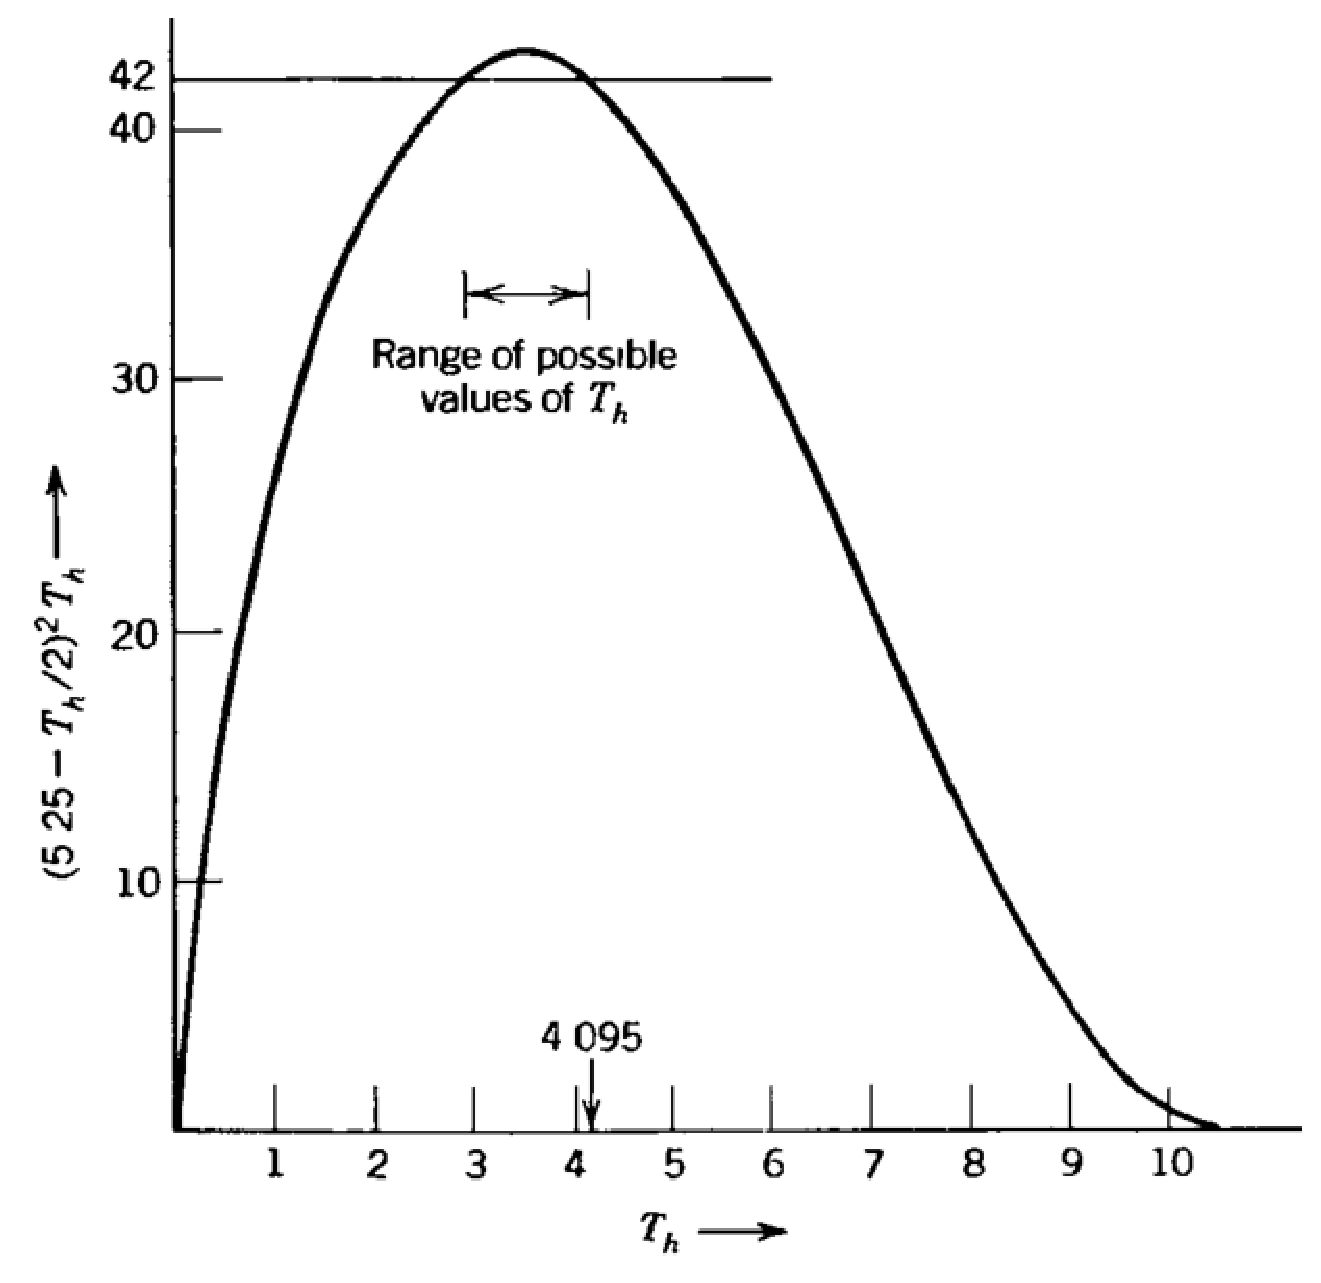
\includegraphics[scale=0.5]{fig4_01.eps} 
}

\subsection*{习题}
\begin{itemize}
\item[4.1-1.] 一摩尔单原子理想气体和一摩尔$c=3/2$的理想 van der Waals 流体(\ref{sec3.5}节)分别装在体积为$v_1$和$v_2$的容器里。理想气体的温度为$T_1$而 van der Waals 流体是$T_2$。我们希望将理想气体的温度变成$T_2$而保持总的能量不变。那么 van der Waals 流体的末温是多少?各参数($T_1,T_2,a,b,v_1,v_2$)之间需要满足什么关系才能实现这样一个温度转换(总是假定在过程中外界不发生改变)?
\item[4.1-2.] 一个橡胶带(\ref{sec3.7}节)初始温度为$T_B$,长度为$L_{B}$。一摩尔单原子理想气体初温为$T_G$,体积为$V_G$。理想气体经历一个定容升温过程达到温度$T_G'$。其所需要的能量全都从橡胶带中获得。那么橡胶带的长度是否需要改变?如果是的话,改变多少?
\begin{flushright}
{\it 答案:}\\
若$l=L_B-L_0$,
\[
l^2-(l')^2\ge 2b^{-1}cL_0(L_1-L_0)\ln\left(1-\frac{3R}{2RL_0}\frac{T_G'-T_G}{T_B}\right)+3Rb^{-1}(L_1-L_0)\ln(T_G'/T_G)
\]
\end{flushright}
\item[4.1-3.] 假设例\ref{eg4.1}中的两个系统热容具有形式$C(T)=DT^n$,其中$n>0$:\\
\begin{enumerate}
\item 证明这样的系统内能$U=U_0+DT^{n+1}/(n+1)$以及熵$S=S_0+DT^n/n$。系统的基本方程是什么?
\item 如果其初始温度分别为$T_{10}$和$T_{20}$,最大可输出功为多少(两系统最后处于相同温度)?
\end{enumerate}
\begin{flushright}
{\it 答案:}\\
对于$n=2$:
\[
W=\frac{D}{3}\left[T_{10}^3+T_{20}^3-\frac{1}{\sqrt{2}}(T_{10}^2+T_{20}^2)^{3/2}\right]
\]
\end{flushright}
\end{itemize}

\section{准静态和绝热过程}\label{sec4.2}
熵极大作为中心原理,当应用于不同类型的过程时能给出不同的定理。我们先重新给出对状态和过程的概念的描述,然后再来关注这些定理。

为了描述一个热力学状态的特征及其可能的过程,有必要引入{\it 热力学构形空间(thermodynamics configuration space)}。一个简单系统的热力学构形空间是由熵和诸广延量$U, V, N_1,\dots ,N_r$坐标轴张成的抽象空间。系统的基本方程$S=S(U, V, N_1,\dots ,N_r)$在热力学构形空间中定义了一个曲面,如图\ref{fig4.1}所示。另外注意图\ref{fig4.1}与$(\partial U/\partial S)_{\dots , X_j,\dots}(\equiv 1/T)$为正,以及$U$是$S_{\dots , X_j,\dots}$的单值函数的要求相符。

{
	\centering
	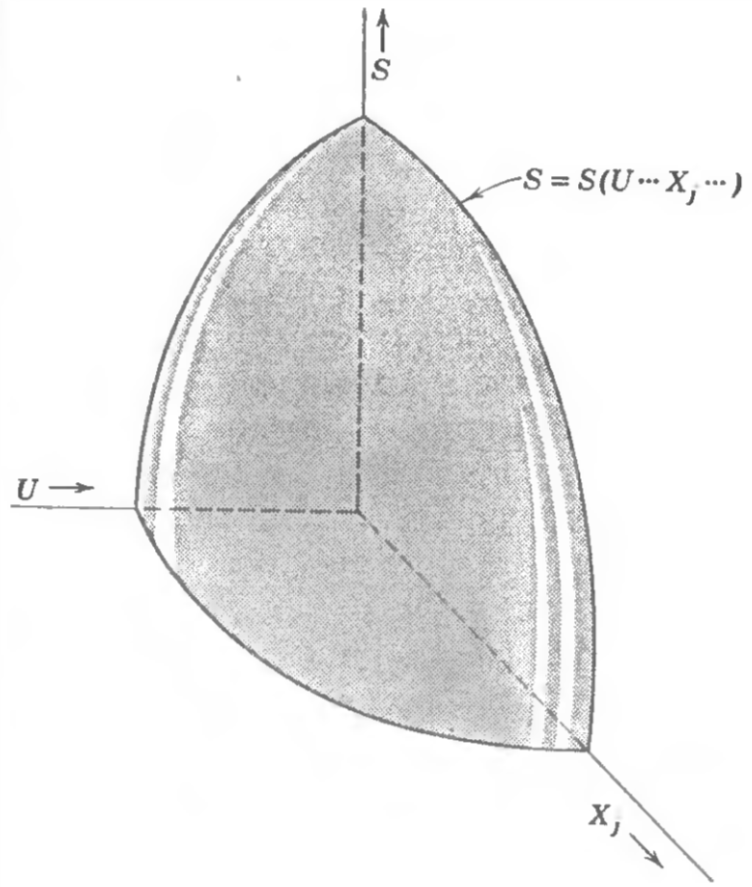
\includegraphics[width=.7\textwidth]{Pictures/fig4.1.png}
	\figcaption{一个简单系统的热力学构形空间中的超曲面$S=S(U, \dots, X_j,\dots)$。}
	\label{fig4.1}
}

根据定义,构形空间中的每一个点代表一个平衡态。而非平衡态需要一个维度大得多的空间中的点来表示。

一个复合体系的基本方程可以由包括了全部子系统的广延量的构形空间中的一张曲面表示。对于含有两个子系统的复合系统,其构形空间的坐标轴应该包括总熵$S$和两个子系统的广延量。一个更方便的选择是总的熵$S$、第一个子系统的广延量$(U^{(1)},V^{(1)},N^{(1)}_1,N^{(1)}_2,\dots)$、以及整个复合系统的广延量$(U,V,N_1,N_2,\dots)$。复合系统构形空间的一个示例见图\ref{fig4.2}。

{
	\centering
	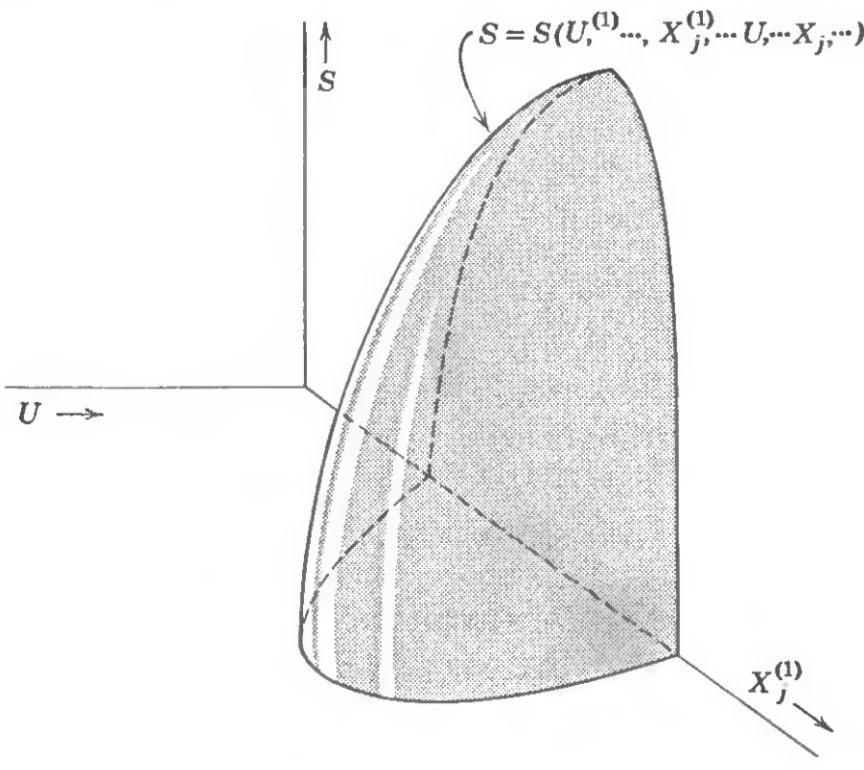
\includegraphics[width=.8\textwidth]{Pictures/fig4.2.png}
	\figcaption{一个复合系统的热力学构形空间中的超曲面$S=S(U^{(1)}, \dots, X^{(1)}_j,\dots,U, \dots, X_j,\dots)$。}
	\label{fig4.2}
}

考虑超曲面上任意一条从初态到末态的曲线,如图 。这样的曲线被称为{\it 准静态轨迹(quasi-static locus)}或{\it 准静态过程(quasi-static process)}。一个准静态过程可以由一连串密集的{\it 平衡}态来定义。值得强调的是,准静态过程是一个理想的概念,而实际过程总是包含着无法在构形空间中表示的非平衡的中间态。另外,相比实际过程,准静态过程从不考虑速率或者时间。准静态过程只是一系列有序的平衡态,而实际过程是一系列在{\it 时间}上有序的平衡态和{\it 非平衡态}。

尽管没有哪个实际过程完全就是准静态过程,但将一个实际过程看作和准静态相近是有可能的。特别的,我们能够让一个系统连续通过给定准静态轨迹上的任意多个点。考虑体系初态处在图\ref{fig4.3}中的$A$点,考察经过点$A, B, C,\dots ,H$的准静态轨迹。现在我们放宽一点约束,允许系统从$A$不经过轨迹上的点运动到$B$。系统从$A$点“消失”,经过一系列无法在图中表示的非平衡态,然后出现在$B$。如果进一步去除约束,使得$C$态也可以到达,系统也会从$B$点消失,然后重新出现在$C$。重复这个操作能让系统到达状态$D,E,\dots ,H$。通过这样一系列实际过程,我们构造了一个近似于图示理想准静态过程的过程。在准静态轨迹上挪动点$A,B,C\dots$,使其间距任意小,我们便可以任意接近于准静态轨迹\mpar{实际上,两个充分接近的平衡态,也可能由一条相当长的非平衡态轨迹所连接。}。

{
	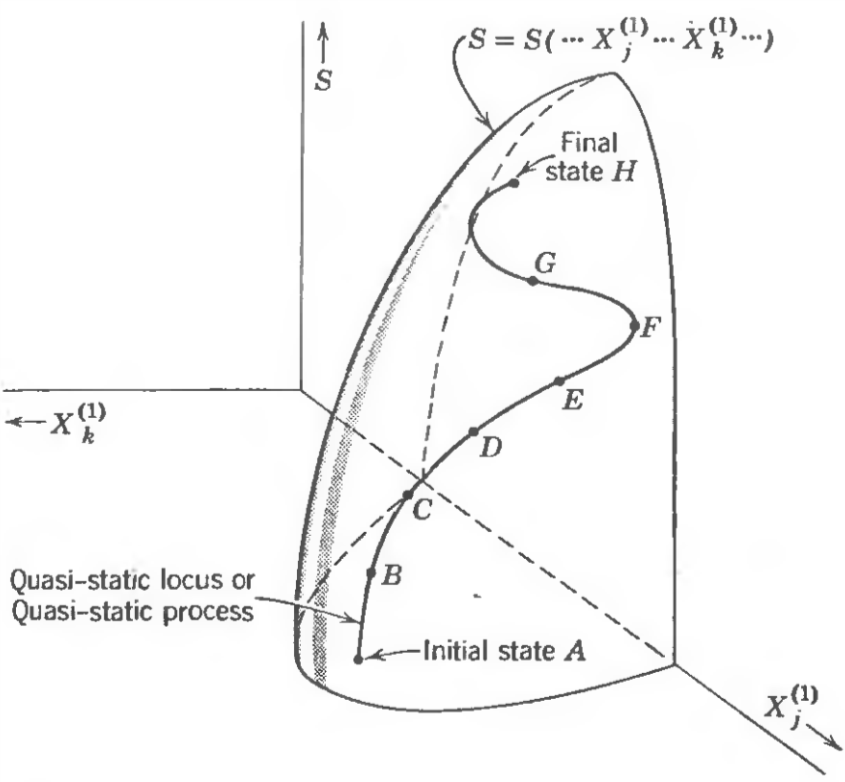
\includegraphics[width=.8\textwidth]{Pictures/fig4.3.png}
	\figcaption{一个准静态过程在热力学构形空间中的表示。}
	\label{fig4.3}
}

{\it $P\,\mathrm dV$作为机械功以及$T\,\mathrm dS$作为热交换的定义仅对准静态过程成立。}

考虑一个{\it 封闭}系统,经历一系列状态$A,B,C,\dots ,H$,近似于一条准静态轨迹。这个系统能在移除一些内部约束后从$A$到$B$。封闭系统能到达$B$当且仅当$B$态在所有可达到的态中有最大的熵值。这里即$B$态的熵比$A$态要高。因此,封闭系统中从$A$态到$B$态的过程是有方向性的。它从一个熵低的态,$A$,到达一个熵高的态$B$,没法倒过来。这样一个过程是{\it 不可逆的(irreversible)}。

{\it 封闭系统的一条准静态轨迹可以由一条实际轨迹近似,仅当轨迹上熵值单调不减。}

{\it 熵增为零的准静态过程被称为可逆过程(reversible process)}(图\ref{fig4.4})。这类过程末态的熵与初态相等,其可以依两个方向移动。

{
	\centering
	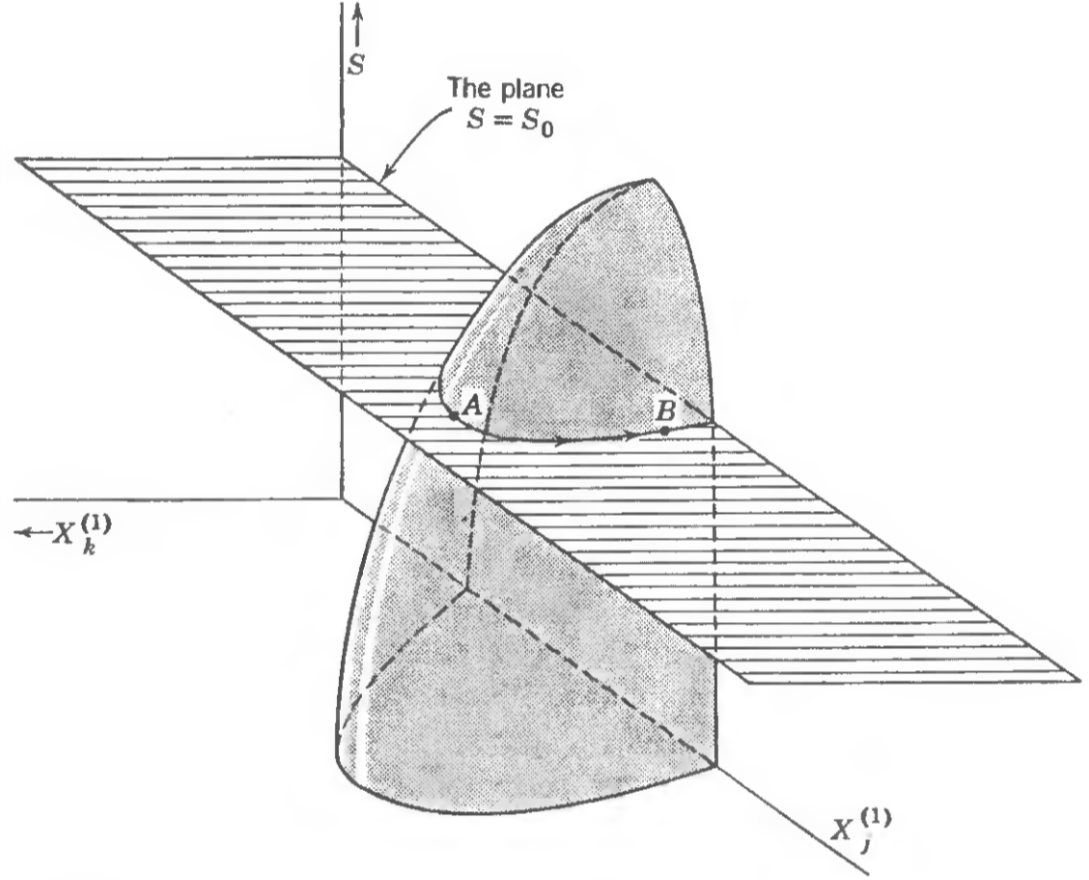
\includegraphics[width=.8\textwidth]{Pictures/fig4.4.png}
	\figcaption{沿着等熵线的可逆过程}
	\label{fig4.4}
}

\subsection*{习题}
\begin{itemize}
\item[4.2-1] 每个可逆过程是否都对应于一条准静态轨迹?每条准静态轨迹是否都对应于一个可逆过程?对于从$A$态到$H$态的任意实际过程,是否存在一些有着同样的两个末态$A$和$H$的准静态过程?是否存在一些有着同样的两个末态$A$和$H$的可逆过程?
\item[4.2-2] 考虑带有活塞的圆柱中的单原子理想气体。圆柱的壁和活塞都是绝热的。系统初始处于平衡态,但外界的压强在缓慢减小。气体的能量由体积膨胀$\mathrm dV$造成的改变为$\mathrm dU=-P\,\mathrm dV$。证明,利用\eqref{equ3.34}式,有$\mathrm dS=0$,即准静态绝热膨胀是等熵且可逆的。
\item[4.2-3] 单原子理想气体由$V$自由膨胀至$V+\mathrm dV$(回忆习题3.4-8)。证明
\[
\mathrm dS = \frac{NR}{V}\mathrm dV
\]
通过这样一系列无穷小自由膨胀,从$V_i$到$V_f$,证明
\[
\Delta S = NR\ln(\frac{V_f}{V_i})
\]
讨论这种非典型(并且臭名昭著的)“连续自由膨胀”过程是否为准静态过程需要一些精细的考虑。作为正面因素,无穷小膨胀的末态可以在轨迹上作到%
\mpar{与初态}%
充分的接近。而作为负面因素,在实现上,系统在每次膨胀中必须经历非平衡态;微膨胀的不可逆性是本质的和不可约的。$\mathrm dS>0$和$\mathrm dQ=0$的事实与对所有准静态过程的假设$\mathrm dQ=T\mathrm dS$相冲突。我们{\it 定义}(某种意义上是循环论证!)连续自由膨胀过程是“本质不可逆的”以及{\it 非准静态的(non-quasi-static)}%
\mpar{另一种解释是,单次自由膨胀这个问题中,外界给原系统添加了另一个子系统——尽管没有能量、粒子数交换。} %
。
\item[4.2-4] 在所考虑的温度范围内,某系统遵循如下方程
\[
T=Av^2/s, \quad P=-2Av\ln(s/s_0)
\]
其中$A$为正常数。这个系统从$v_0$自由膨胀至$v_f$($v_f>v_0$)。求体系的末温$T_f$关于初温$T_0$,以及$v_0,v_f$的函数。求摩尔熵的增量。
\end{itemize}

\section{弛豫时间和不可逆性}\label{sec4.3}
考虑依图\ref{fig4.3}所示准静态轨迹行进的系统。随着约束一步一步的被移除,系统逐步历经轨迹上各个平衡态。每当放松一个约束,我们就得等待一段时间,使系统达到平衡态,然后再放松下一个约束,以此往复。尽管在理论上是这样规定的,但实际执行起来却很少按着这个模式来。实践上,约束常是连续地,在“充分慢”的速度下解除的。

为了得到一条足够像的准静态轨迹,其所要求的解除约束的速度可以用系统的{\it 弛豫时间(relaxation time)}\, $\tau$来表征。对于一个给定弛豫时间$\tau$的系统,在少于时间$\tau$内发生的过程是非准静态的,而长于时间$\tau$的过程可以近似看作准静态的。

如何从物理上估计一个系统的弛豫时间呢?我们可以从气体的绝热膨胀中得到启发(回忆习题4.2-2)。如果那个活塞只能极慢地向外移动,那么过程便是准静态的(且是可逆的)。如果,外压下降地非常快,致使活塞迅速移动,并伴随着圆柱里的气体紊乱的流动(熵增“驱使”着此过程)。那么,这个过程便即不是准静态的,也不是可逆的。为了估计弛豫时间,我们先注意到活塞向外的一个微小位移将会马上减小与活塞相邻气体的密度。如果这个膨胀是可逆的,那么这个局部的气体“稀疏区”会在活塞再次移动可观的距离之前被气流所抹平。稀疏区自身会在气体中以声速传播,在容器壁上反射,并逐渐消失。消失来自于壁的漫反射和气体的粘滞阻力。最简单的情形大概就是圆柱的壁足够粗糙,以至于一次反射就足以耗散掉稀疏区的脉冲——尽管这不是普遍情况,但也足以达到我们作启发性思考的目的了。那么弛豫时间就将是稀疏区传播穿过整个系统的时间$\tau\approx V^{1/3}/c$,其中体积的三次方根代表系统的“尺度”,而$c$为气体中的声速%
\mpar{有趣的是,不少教材中声速的推导需要用到准静态过程的假定。}%
。如果气体绝热膨胀是在远大于弛豫时间的时间内发生的,那么这个膨胀便是可逆且等熵的。如果膨胀是在短于或相当于弛豫时间的时间内发生的,那么系统将会面对不可逆的熵增,膨胀便是绝热但不等熵的。

\subsection*{习题}
\begin{itemize}
\item[4.3-1] 一个长为$L$,横截面积为$A$的圆柱形容器,被由一个螺钉固定的活塞分为两个等体积的气室。一个气室包含$N$摩尔温度为$T_0$的单原子理想气体。活塞与这个气室的壁之间由一个原长为$L/2$的弹簧连接,即当活塞位于初始位置时,没有额外的力作用在其上。弹簧的劲度系数为$K_\text{spring}$。容器的另一个腔体被抽成真空。突然撤去螺钉。试求气体最终达到平衡态时的体积和温度。假定腔壁和活塞是绝热的,弹簧、活塞和腔壁的热容可以忽略。\\
讨论导致这个最终平衡态的过程。如果容器中每个腔体中都盛有气体,则终态将会是不确定的!为什么?
\end{itemize}

\section{热流:耦合系统和逆过程}
\label{sec4.4}
最典型的热力学过程大概就是两个系统之间的热传导了,仔细考察这个过程将会是富有教益的。

考虑最简单的情形,热量$\dbar Q$从温度为$T$的一个系统转移到{\it 相同}温度的另一个系统。这样的过程是可逆的,接受热量的子系统的熵增$\dbar Q/T$正好会被吸收热量的子系统的熵减$-\dbar Q/T$抵消。

作为对比,假定两个子系统有不同的初始温度$T_{10}$和$T_{20}$,且$T_{10}<T_{20}$,其(定容)热容分别为$C_1(T)$和$C_2(T)$。如果$\dbar Q$的热量准静态的流入系统1(体积不变),其熵增为
\begin{equation}
\mathrm dS_1 = \frac{\dbar Q_1}{T_1} = C_1(T_1)\frac{\mathrm dT_1}{T_1},
\end{equation}
对于系统2是类似的。如果这样无穷小的热传导过程一直进行,直到两个物体温度相等,那么能量守恒要求
\begin{equation}
\Delta U = \int_{T_{10}}^{T_f} C_1(T_1)\,\mathrm dT_1 + \int_{T_{20}}^{T_f}C_2(T_2)\,\mathrm dT_2 = 0,
\end{equation}
依此确定$T_f$。总的熵变为
\begin{equation}
\Delta S = \int_{T_{10}}^{T_f} \frac{C_1(T_1)}{T_1}\,\mathrm dT_1 + \int_{T_{20}}^{T_f}\frac{C_2(T_2)}{T_2}\,\mathrm dT_2
\end{equation}

对于热容$C_1,C_2$与温度无关的情形,能量守恒式变为
\begin{equation}
T_f = \frac{C_1T_{10}+C_2T_{20}}{C_1+C_2}
\end{equation}
熵增为
\begin{equation}
\Delta S = C_1\ln\left(\frac{T_f}{T_{10}}\right) + C_2\ln\left(\frac{T_f}{T_{20}}\right)
\label{equ4.5}
\end{equation}
$\Delta S$大于零的证明留作习题。

我们需要从几个不同角度再回顾一下热传导过程。

首先需要注意到这个过程虽然是准静态的,但不是可逆的:它在热力学构形空间中由一条熵单调增的准静态轨迹代表。

其次,对于热量从热系统传递到冷系统,这个准静态过程可以在如下条件下{\it 自发}进行:(1)两系统之间传导热量的壁足够薄以致于其质量(以及其对体系热力学性质的影响)可以忽略;(2)热量传导的速率足够慢(例如,壁的热阻足够高)使得每个子系统内部温度都是均匀的。

最后,我们注意到一个子系统的熵是{\it 下降}地,而另一子系统的熵上升。{\it 使任何特定系统的熵降低都是可行的,但是这会导致其他某些系统更高的熵增。}这个对于单个系统的不可逆过程,可以变得“可逆”——{\it 当然总得在某个犄角旮旯里付出代价}。

{\bf 习题}
\begin{itemize}
\item[4.4-1] 两个物体在所考虑的温度区间内都具有如下的热容形式
\begin{equation*}
C=A+BT
\end{equation*}
其中$A=\SI{8}{\joule/\kelvin}$,$B=\SI{2e-2}{\joule/\kelvin^2}$。如果两物体初始温度分别为$T_{10}=\SI{400}{\kelvin}$和$T_{20}=\SI{200}{\kelvin}$,使其作热接触,试问末温和熵变。
\item[4.4-2] 考虑习题4.4-1中的系统,再加入第三个物体,其热容为
\begin{equation*}
C_3=BT
\end{equation*}
初始温度为$T_{30}$。物体一和物体二相互隔开,物体三与物体二作热接触。为了使得物体二回到初态,$T_{30}$得是多少?第二个过程中物体二减少了多少的熵?
\item[4.4-3] 证明式\eqref{equ4.5}给出的熵增总是正的。
\item[4.4-4] 证明,对于两个有相同常数热容的物体,其直接热接触得到的末态平衡温度等于两物体初温的代数平均。
\item[4.4-5] 在所考虑的温度范围内,某类系统的定体热容量反比于温度。
	\begin{itemize}
	\item[a)] 定体情况下,这类系统的能量与温度的关系如何?
	\item[b)] 如果两个这样的系统,初温分别为$T_{10}$和$T_{20}$,相互作热接触,其最终平衡温度为多少?
	\end{itemize}
\item[4.4-6] $N+1$缸水排成一排,其初始温度分别为$T_0,T_1,T_2,\dots,T_N$(有$T_n>T_{n-1}$)。一个小物体定体热容为常数$C$,初态与$T_0$的那缸水达到热平衡。随后将物体浸在温度为$T_1$的缸里。这个过程反复$N$次,直到物体与温度为$T_N$的缸达到热平衡。假定相邻两缸水的温度之比为常数,即
\begin{equation*}
T_n/T_{n-1} = (T_N/T_0)^{1/N}
\end{equation*}
并且略去每一缸水的(微小)温度变化,计算如下两种过程的熵增:
	\begin{itemize}
	\item[a)] 物体被“升序”移动(从$T_0$到$T_N$)
	\item[b)] 物体被“降序”带回(从$T_N$到$T_0$)。
	\end{itemize}
计算熵增在$N\rightarrow \infty$时的领头项,$T_0,T_N$保持为常数。注意到对于大$N$有如下展开式
\begin{equation*}
N(x^{1/N}-1)=\ln x+(\ln x)^2/2N+\dots
\end{equation*}
\end{itemize}


\section{最大功定理}
\label{sec4.5}
可以利用物理系统倾向于熵增大的性质性质来做功,所有此类应用都遵循最大功定理。

考虑一个初态与末态确定的系统(称为主系统\mpar{原文为“subsystem”(子系统),这里翻译成“主系统”,这样能强调它在总体$\{ \text{subsystem, 可逆热源,可逆功源} \}$当中的主体地位。})。与两个附加系统,一个可以与主系统交换功,一个可以与主系统交换热。最大功定理指出,{\it 对于主系统从初态变为末态的所有可能过程而言,在可逆过程中主系统做功最大(放热最小)}。而且{\it 对于任一可逆过程,主系统做功(传热)是相等的。}

与主系统交换功的“仓库”系统称为“可逆功源”\mpar{reversible work source, 下文常用\text{RWS}指代。}。可逆功源定义为{\it 由绝热且不可渗透(不能进行物质交换)的器壁围成的、弛豫时间足够小以至于其中发生的所有过程都可以视为准静态的系统}。从热力学的观点来看,力学中的“保守”(非耗散)系统都是可逆功源。

与主系统交换热的“仓库”系统被称为“可逆热源”\footnote{源这个字的使用可能使大家倾向于认为主系统从其中吸取而不是向其中释放热量,这种差别是不存在的}。\mpar{reversible heat source, 下文常用\text{RHS}指代。}可逆热源定义为{\it 由刚性且不可渗透器壁围成的、弛豫时间足够小以至于其中发生的所有过程都可以视为准静态过程的系统}。如果可逆热源的温度为$T$,由准静态关系$\dbar Q = T\rd S$交换给可逆热源的热量$\dbar Q$会使它的的熵增大。可逆热源与外界的相互作用可以由它的热容$C(T)$完全描述(可逆热源的定义表明它的热容只能为等容热容,所以不必用下标标出)。可逆热源内能的变化为$\rd U = \dbar Q = C(T) \rd T$,熵的变化为$\rd S = [C(T)/T] \rd T$。最大功定理中涉及的各种传递过程都在图4.5中标示出。

{
	\centering
	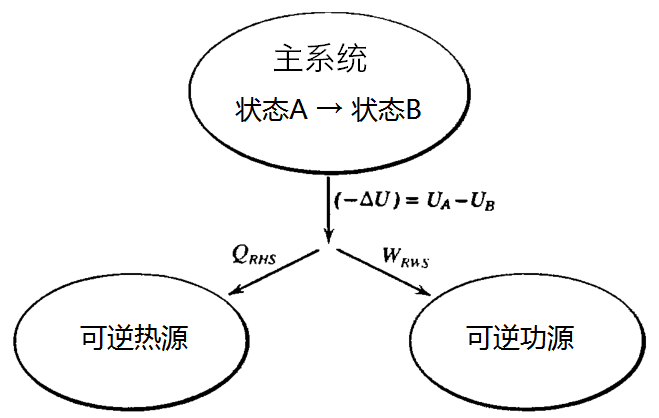
\includegraphics[scale=0.6]{fig4_5.png}
	\figcaption{最大功过程示意图。最大功过程是可逆的$(\Delta S_{\text{total}} = 0)$,主系统对可逆功源做的功$W_{\text{RWS}}$最大、传给可逆热源的热量$Q_{\text{RHS}}$最小。}
}

最大功定理的证明是直接的。考虑两个过程。每个过程都使主系统产生相同的内能变化$\Delta U$和熵的变化$\Delta S$,因为这些都是由主系统钦定的初态和末态决定的。两个过程不同之处仅仅在于主系统初态与末态的内能之差($-\Delta U$)在可逆功源与可逆热源之间的分配($-\Delta U = W_{\text{RWS}} + Q_{\text{RHS}}$)。向可逆功源做功最大同时也相应地向可逆热源放热最少的的过程,自然就是引起可逆热源熵的变化最小的过程(因此也是整个系统熵变最小的过程,因为可逆功源的熵变为零、主系统的熵变确定)。

在{\it 所有}可能的过程中,{\it 任何一个}可逆过程都可以达到$\Delta S_{\text{total}}$的绝对最小值。(对于所有的可逆过程都有$\Delta S_{\text{total}} = 0$)。

简而言之,能量守恒要求$\Delta U + W_{\text{RWS}} + Q_{\text{RHS}} = 0$。 $\Delta U$确定,要使$W_{\text{RWS}}$最大则应该使$Q_{\text{RHS}}$最小。这可以通过使$S^{\text{final}}_{\text{RHS}}$最小来实现(因为$S_{\text{RHS}}$随可逆热源的吸热$Q_{\text{RHS}} > 0$单调增加)。而$S^{\text{final}}_{\text{RHS}}$的最小值则通过使$S_{\text{total}}$最小,或者说$S_{\text{total}} = 0$来取得。

上述“描述性的”证明可以转化为更规范的语言,当主系统的初态和末态十分接近,它们之间的所有差别都可以用微分来表达时,这种转化显得尤为具有启发性。能量守恒要求
\begin{equation}
\label{equ4.6}
\rd U + \dbar Q_{\text{RHS}} + \dbar W_{\text{RWS}} = 0
\end{equation}
而熵增原理要求
\begin{equation}
\label{equ4.7}
\rd S_{\text{tot}} = \rd S + \frac{\dbar Q_{\text{RHS}}}{T_{\text{RHS}} } \ge 0
\end{equation}
由此可知
\begin{equation}
\label{equ4.8}
\dbar W_{\text{RWS}} \le T_{\text{RHS}} \rd S - \rd U 
\end{equation}
不等式右边的量都是定值。$\rd S$和$\rd U$分别是是主系统钦定的初态和末态之间的熵之差与内能之差。最大功$\dbar W_{\text{RWS}}$对应于\eqref{equ4.8}中等号成立的情况,也即\eqref{equ4.7}中等号成立的情况($\rd S_{\text{tot}} = 0$)。

计算出最大功是很有用的,从\eqref{equ4.8}和等量关系$\rd U = \dbar Q + \dbar W$中,得到
\begin{equation}
\label{equ4.9}
\begin{split}
\dbar W_{\text{RWS}} (\text{maximum}) &= \left( \frac{T_{\text{RHS}}}{T} \right) \dbar Q - \rd U \\
&= \left[ 1 - \left( \frac{T_{\text{RHS}}}{T} \right) \right] (-\dbar Q) + (-\dbar W)
\end{split}
\end{equation} 
也就是说,{\it 在无穷小过程中,能对可逆功源所做的最大功为以下二者之和:

\begin{enumerate}
\item[(a)] 主系统对外做功($-\dbar W$),  
\item[(b)] 主系统释放热量($-\dbar Q$)的($1 - T_{\text{RHS}}/T$)倍。
\end{enumerate}}
占主系统释放热量总量($1 - T_{\text{RHS}}/T$)的热量可以在无穷小过程中“转化”为功,这个分数称为{\it 热机效率 (thermodynamic engine efficiency)},\ref{sec4.5}节会继续讨论这个物理量。但是,{\it 我们往往更倾向于依据过程中内能变化和熵变的总量来解决最大功问题}(而不采用算出微小过程的热机效率然后对全过程积分)。

回到整个(非无穷小)过程,能量守恒条件变为
\begin{equation}
\label{equ4.10}
\Delta U_{\text{主系统}}+Q_{\text{RHS}}+W_{\text{RWS}}=0
\end{equation}
可逆性条件为
\begin{equation}
\label{equ4.11}
\Delta S_{\text{total}} = \Delta S_{\text{主系统}} + \int \frac{\dbar Q_{\text{RHS}}}{T_{\text{RHS}}} = 0
\end{equation}
计算方程中的积分必须要知道可逆热源的热容$C_{\text{RHS}}(T)=\dbar Q_{\text{RHS}}/\rd T_{\text{RHS}}$. 给定$C_{\text{RHS}}(T)$就可以计算出这个积分,进而可以推断净热交换$Q_{\text{RHS}}$. 反过来根据\eqref{equ4.10}式又可以算出$W_{\text{RWS}}$. {\it 利用\eqref{equ4.10}和\eqref{equ4.11}式,通过上述程序计算,就可以解决最大功定理相关的所有问题。}

如果可逆热源是一个{\it 热库},那么问题将会进一步简化。热库的是很大的可逆热源,大到我们所关心的任何热交换都可以视为不改变其温度。简而言之,热库就是具有{\it 固定}并且明确温度的热源。对于这样一个系统,\eqref{equ4.11}式简化为
\begin{equation}
\label{equ4.12}
\Delta S_{\text{total}} = \Delta S_{\text{主系统}}+\frac{Q_{\text{热库}}}{T_{\text{热库}}}
\end{equation}
并且通过\eqref{equ4.10}和\eqref{equ4.12}式可以消去$Q_{\text{热库}}(=Q_{\text{RHS}})$, 得到\mpar{由于已经使用了可逆性条件$\Delta S_{\text{total}} = 0$,故下式中的$W_{\text{RWS}}$为主系统对可逆热源做的最大功。}
\begin{equation}
\label{equ4.13}
W_{\text{RWS}}=T_{\text{热库}} \Delta S_{\text{主系统}}-\Delta U_{\text{主系统}}
\end{equation}
最后指出,主系统钦定的末态的能量是可以比初态更大的。在那种情况下最大功定理仍然成立,但是主系统“对外做功”应该为负。(所以根据最大功定理)对于可逆过程而言这份对主系统所做的功是最小的(此时主系统对外做功仍然是其代数最大值)。

\textbf{例 1}
一摩尔理想van der Waals流体经过某个过程从初态$T_0$,$v_0$变为末态$T_f$,$v_f$。另一个系统(作为可逆热源)有确定的体积和初始温度$T_{20}$;它的热容随温度线性变化:
\[C_2(T)=DT \quad (D=\text{constant})\]
系统对可逆功源做的最大功是多少?

\paragraph{解} 这个问题与\ref{sec4.1}节中的例题的解法相似,只是公式有所不同。第二个系统是一个可逆热源;因此能量对温度的依赖关系为
\[U_2(T)=\int C_2(T)\text{d}T=\frac{1}{2}DT^2 + \text{constant}\]
熵对温度的依赖关系为
\[S_2(T)=\int\frac{C_2(T)}{T}\text{d}T=DT + \text{constant}\]

因为理想van der Waals流体系统的能量和熵对于$T$和$v$的依赖关系由\eqref{equ3.49}和\eqref{equ3.51}式给出,从中可得
\[\Delta U_1 = cR(T_f - T_0) -\frac{a}{v_f} + \frac{a}{v_0}\]
\[\Delta S_1 = R\ln \left(\frac{v_f-b}{v_0-b} \right) + cR\ln\frac{T_f}{T_0}\]
第二个系统(可逆热源)的温度从$T_{20}$变为某个未知的温度$T_{2f}$,所以
\[\Delta U_2 = \frac{1}{2}D(T^2_{2f} - T^2_{20})\]
并且
\[\Delta S_2 = D(T_{2f} - T_{20})\]
$T_{2f}$的值由可逆性条件决定
\[
	\Delta S_1 + \Delta S_2 = R \ln \left( \frac{v_f - b}{v_0 - b} \right) + cR \ln \frac{T_f}{T_0} + D(T_{2f} - T_{20}) = 0
\]
上式变形为
\[
	T_{2f} = T_{20} - RD^{-1} \ln \left( \frac{v_f - b}{v_0 - b} \right) - cRD^{-1} \ln \frac{T_f}{T_0}
\]

能量守恒条件要求主系统对可逆功源所做的功$W_3$满足
\[W_3 + \Delta U_2 + \Delta U_1 = 0\]
由此
\[W_3 = -\Big[ \frac{1}{2} D(T^2_{2f} - T^2_{20}) \Big] - \Big[cR(T_f - T_0)-\frac{a}{v_f}+\frac{a}{v_0} \Big] \]
其中$T_f$已知, $T_{2f}$在上文已求出。

习题4.5-1讨论了一个更简单系统(单原子理想气体和热库)的相似问题。解决这两个问题不需要任何使系统从初态变为末态的具体过程,但习题4.5-2中涉及到了特定的过程(习题4.5-2和4.5-1强烈推荐给读者)。

\textbf{例 2 \quad 同位素分离}

在分离\ce{U^{235}}和\ce{U^{238}}以生产原子能发电站所需的浓缩燃料的过程中天然的铀与氟反应生成六氟化铀(\ce{UF_6})。六氟化铀在室温和大气压下是气体。天然的铀中\ce{U^{235}}摩尔分数$0.0072$,即$0.72 \%$。生产$1$摩尔$2 \%$的浓缩燃料需要加工$10$摩尔天然的\ce{UF_6},剩余$9$摩尔废料。\ce{UF_6}气体可以近似视为一种多原子、多组分的简单理想气体,$c = 7/2$(\eqref{equ3.40}式)。假定分离过程在温度为\SI{300}{K},压强为一个大气压的条件下进行,并且假定外界大气为热库(温度为\SI{300}{K}),那么进行浓缩过程所需的最小功是多少?这些功(能量)最终去了哪里?

\paragraph{解} 这个问题是一个最大功原理的实例,其中系统{\it 所需的}最小功对应于系统“所做的”最大功。系统的初始状态为$10$摩尔天然\ce{UF_6},$T = \SI{300}{K}$,$P = \SI{1}{atm}$。系统的末态为相同温度与压强下的1摩尔浓缩气和9摩尔废气。冷库(外界大气)也处于相同的温度。

我们需要找到系统的熵变和内能变化。由条件可知,系统的状态方程是熟悉的形式:
\[U = 7/2NRT. \quad PV = NRT\]
根据\eqref{equ3.40}式可以写出系统的基本方程,联立就能够将熵写成$T$和$P$的函数:
\[S = \sum_{j=1}^2 N_j s_{0j} + \left( \frac{7}{2} \right) NR \ln \left( \frac{T}{T_0} \right) - NR \ln \left( \frac{P}{P_0} \right)- NR \sum_{j=1}^2  x_j \ln x_j\]
最后一项——“混合熵”如\eqref{equ3.40}式所定义,是同位素分离过程至关重要的一项。

首先计算在$9$摩尔废料中\ce{U^{235} F_6}的摩尔分数;经计算得出为$0.578 \%$。由此系统熵变为
\[
\begin{split}
	\Delta S = & \underbrace{ -R[0.02 \ln 0.02 + 0.98 \ln 0.98] }_{\SI{1}{mol}\text{浓缩气} } - \underbrace{ 9R[0.00578 \ln 0.00578 + 0.994 \ln 0.994] }_{ \SI{9}{mol}\text{废气} } \\
	&+ 10R[ \underbrace{ 0.0072 \ln 0.0072 }_{\SI{10}{mol} \text{天然气体中\ce{U^{235}F_6}部分 } } + \underbrace{ 0.9928 \ln 0.9928 }_{ \ce{U^{238}F_6} \text{部分} } ] = -0.0081R \\
	=& -\SI{0.067}{J/K} 
\end{split}
\]
气体{\it 放热}。

气体的能量没有变化,所有对系统所做的功都通过热量传递给了外界大气。这份功,或者说热量,为
\[-W_{\text{RWS}} = Q_{\text{热库}} = -T\Delta S = 300 \times 0.067 = \SI{20}{J} \]

如果存在一种半透膜,\ce{U^{235}F_6}能透过,但是\ce{U^{238}F_6}不能通过,那么分离就能轻易完成。不幸的是这种半透膜不存在。实际中采用的分离方法都是利用两种同位素细微的质量差异的动态(非准静态)过程——利用离心器,质谱仪或者气体扩散。

\section{热机、制冷机和热泵的工作功率}\label{sec4.6}
从\eqref{equ4.6}和\eqref{equ4.7}式可知,在包含了一个“热”的主系统、一个“冷”的可逆热源和一个可逆功源的无限小可逆过程中,有
\begin{equation}
(\dbar Q_h+\dbar W_h)+\dbar Q_c+ \dbar W_\text{\text{RWS}} = 0
\label{equ4.14}
\end{equation}
以及
\begin{equation}
\rd S_h + \frac{\dbar Q_c}{T_c} = 0
\label{equ4.15}
\end{equation}
其中下标$h$代表“热”系统,下标$c$代表“冷”系统。在这样一个过程中所做功$\dbar W_\text{\text{RWS}}$达到了代数意义上的最大值。这能对许多有用设备的操作给出判据。

{\it 热机(thermodynamic engine)}便是最直接的应用。此处的“热系统”可能是某个熔炉或者蒸汽锅炉,而“冷”的可逆热源也许是环境大气,对于发电站来说大概是河流和湖泊。效率被定义为从热系统流出的热量%
\footnote{这里的符号可能会引起一些误解。整本书中,符号$W$和$Q$,或者$\dbar W$和$\dbar Q$代表{\it 输入}系统的功和热量。那么流出系统的便是$(-Q)$或$(-\dbar Q)$。这样{\it 流出}热系统的\SI{5}{\joule}热量会写成{\it 输出}$(-Q_h)=\SI{5}{\joule}$,而热量{\it 输入}为$Q_h=\SI{-5}{\joule}$。为了清楚起见,在这一章中,我们附加了额外的括号用以提醒在这个例子中$(-Q_h)$是一个正的值。}%
$(-\dbar Q)$转化成功$\dbar W_\text{\text{RWS}}$的比例。令\eqref{equ4.14}式中$\dbar W_h=0$(这仅是\eqref{equ4.9}式中加在做功上的一项)\mpar{即认为热机的主系统(例如锅炉)只通过释放热量转化为功},我们可以得到{\it 热机效率(thermodynamic engine efficiency)}\ $\varepsilon_e$:
\begin{equation}
\varepsilon_e = \frac{\dbar W_\text{\text{RWS}}}{(-\dbar Q_h)} = 1 - \frac{T_c}{T_h} 
\label{equ4.16}
\end{equation}
能量交换的关系如图\ref{fig4.6}a所示。

{
	\centering
	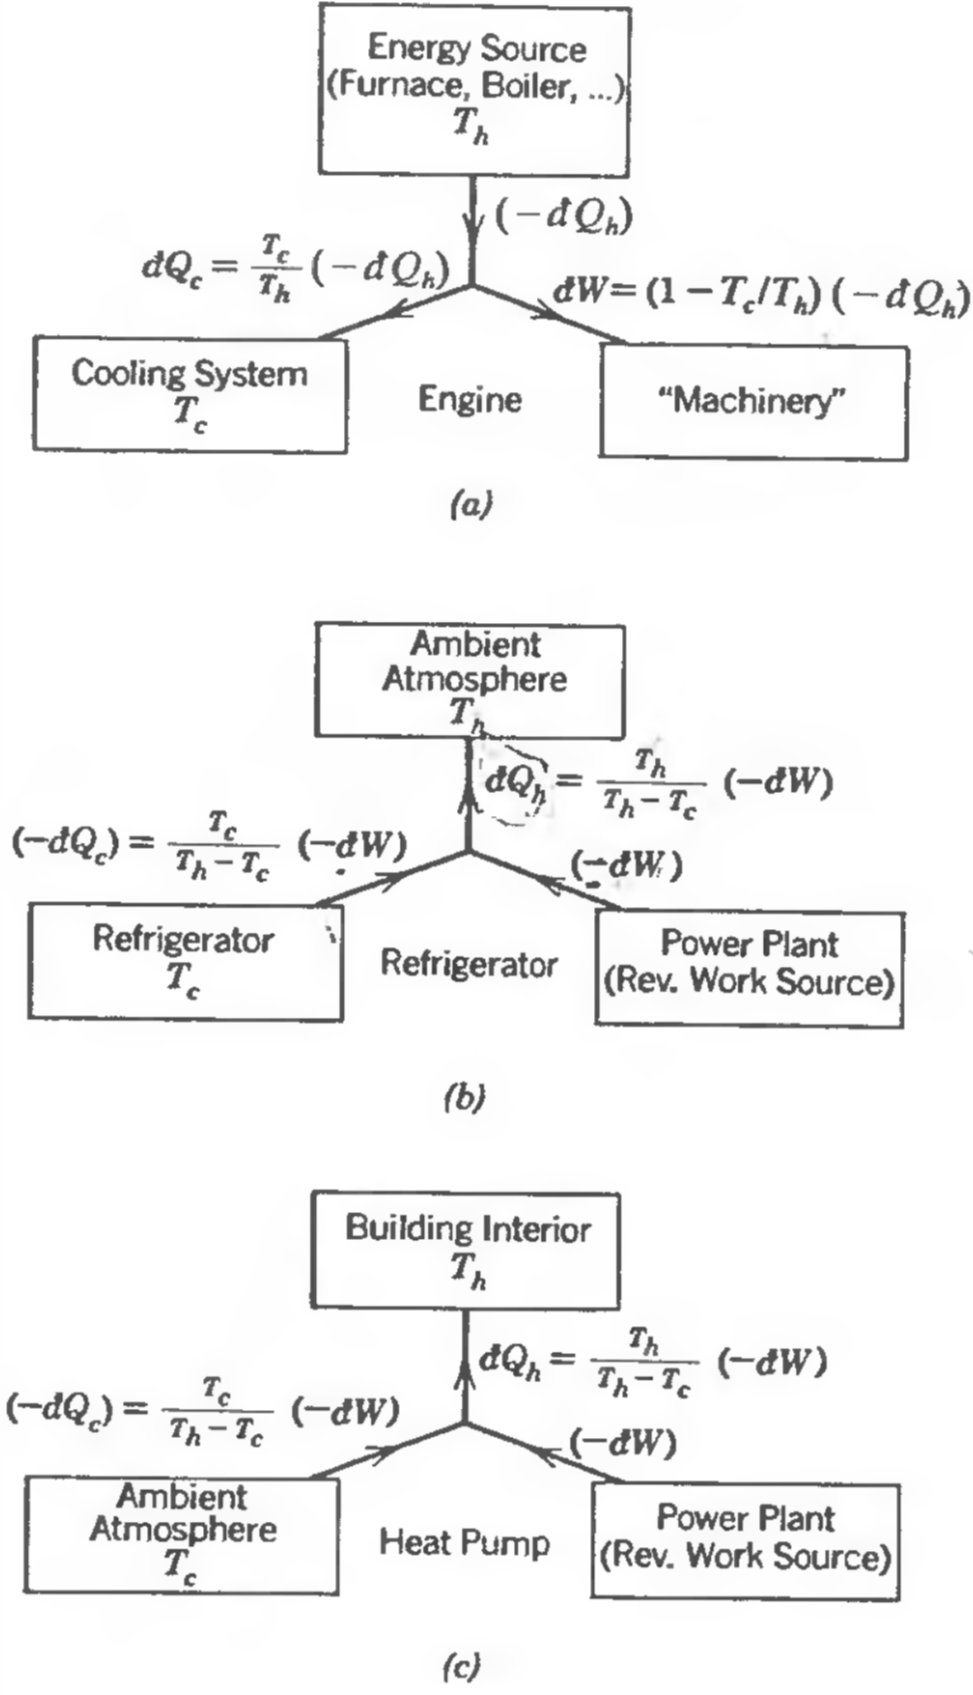
\includegraphics[width=.5\textwidth]{Pictures/fig4.6.png}
	\figcaption{热机、制冷机和热泵。图中有$\dbar W=\dbar W_{\text{RWS}}$}
	\label{fig4.6}
}

若主系统温度$T_h$给定,热机效率随$T_c$降低而升高。即冷系统(热量流向的地方)的温度越低,热机效率越高。理论上最大的效率为$1$,当低温端温度为零时达到。如果有一个零温的水库可以作为低温热源,那么热量变可以完全转变成功(再也不用需要担心“能源危机”%
\footnote{能源短缺,在任何意义上都不是一个恰当的词。能量是守恒的!缺的是“熵汇”——低熵系统。有了这样的系统,我们便可以和大自然作交易,升高它们的熵(通过氧化碳氢化合物、使热量流向低温热源或者使气体膨胀),去完成有用的任务。我们面临的是“负熵短缺”!}%
\mpar{英文原文为"energy shortage",中文直译作能源短缺,某种意义上倒是避免了这个问题。}%
了!)。

{\it 制冷机/冰箱(refrigerator)}就是倒过来运转的热机。这个设备是用来通过耗费尽量少的功来将热量从一个冷系统中提取出释放到相对较热的环境大气中的。\eqref{equ4.14}式和\eqref{equ4.15}式依旧管用,但{\it 制冷机的工作效率(coefficient of refrigerator performance)}得恰当的反映出这个设备的目的——其定义为制冷机从冷系统中吸收的热量与从电力公司买来的电做功之比
\begin{equation}
\varepsilon_r \equiv \frac{(-\dbar Q_c)}{(-\dbar W_\text{\text{RWS}})} = \frac{T_c}{T_h-T_c}
\end{equation}

如果$T_c=T_h$,则制冷机的工作效率将变为无穷大:不需要做功就能将热量从一个系统转移到另一个系统。当$T_c$相对$T_h$下降时,效率会降低。如果$T_c$达到零,则工作效率也将为零(假定$T_h$不变)。即便是将很少的热量从一个零温附近的系统中提取出来,也需要消耗大量的功。

现在考虑{\it 热泵(heat pump)},它通过可逆功源做功从低温热源处提取热量来加热高温系统。一个实际的例子是,在大冬天,你家里是高温系统,户外是低温热源,而可逆功源还是电力公司。实际上,热泵加热房间的原理相当于把冰箱的门打开,让它对着窗户外。冰箱里和室外联通了,它就会尝试(尽管不可能成功)继续给室外降温。从这个巨大的热源中提取的热量,加上这个过程所消耗的从电力公司买来的能量,一起通过冰箱的冷凝管传到了室内。

{\it 热泵的工作效率(coefficient of heat pump performance)}\ $\varepsilon_p$定义为流入热系统的热量与所做功之比:
\begin{equation}
\varepsilon_p \equiv \frac{\dbar Q}{(-\dbar W_\text{\text{RWS}})} = \frac{T_h}{T_h-T_c}
\end{equation}

{\bf 习题}
\begin{itemize}
\item[4.6-1] \SI{0.001}{\kelvin}是实验室中较容易达到的温度。如果电力公司的电价是\SI{15}[\$]{\per\kilo\watt\per\hour},那么从温度为\SI{0.001}{\kelvin}的系统中提取一瓦时的热量需要花多少钱?高温热源为\SI{300}{\kelvin}的环境大气。
\begin{flushright}
{\it 答案:}\\ \SI{45}[\$]{}
\end{flushright}
\item[4.6-2] 一个房间维持在\SI{70}{\degreeF},而室外为\SI{50}{\degreeF}。一个加热房间的办法是将从电力公司买来的功直接转换成热,这也是许多电热器所用的策略。另一种办法是用这些功来驱动一个热泵。如果这个热泵能达到理想的工作效率,那么耗费比是多少?
\item[4.6-3] 一个家用冰箱的内部温度为\SI{35}{\degreeF}。每开关一次冰箱门放个什么东西进来,会带来平均\SI{50}{\kilo\calorie}的热量,但几乎不改变冰箱的温度。冰箱每天开关15次,并以理想工作效率的 15\% 工作。电价是\SI{15}[\$]{\per\kilo\watt\per\hour}。试问为这台冰箱每月该付多少钱?
\item[4.6-4] 从\SI{4.2}{\kelvin}的液氦中抽取热量,高温端为\SI{77.3}{\kelvin}的液氮。问每从液氦中抽取一 joule 热量,会向液氮中传递多少 joule 热量?
\item[4.6-5] 假定某物体具有状态方程$U=NCT$,其中$NC=\SI{5}{\joule\per\kelvin}$,其在\SI{0.5}{\kelvin}至室温的范围内适用。以环境大气作为高温热源,需要花费多少功才能将该物体从室温(\SI{300}{\kelvin})降至\SI{0.5}{\kelvin}?
\begin{flushright}
{\it 答案:}\\ \SI{16.2}{\kilo\joule}
\end{flushright}
\item[4.6-6] 一摩尔单原子理想气体等温的从10升膨胀15升,其温度为\SI{400}{\kelvin}。这个过程所作功被用来驱动工作在\SI{200}{\kelvin}和\SI{300}{\kelvin}之间的制冷机。其最多可以在低温端带走多少热量?
\item[4.6-7] 给出\ref{sec4.1}节中例\ref{eg4.2}的一个构造性的解。你为使高温物体温度达到最高的解,可以基于以下过程:两个较冷物体间工作的热机,工作直至两物体等温。其所作的功用以驱动一个热泵,工作与低温物体对与高温物体之间。证明这个过程能得到原例中相同的结果。
\item[4.6-8] 假定一摩尔理想van der Waals 流体等温膨胀,温度为$T_h$,体积由初态$V_i$膨胀至$V_f$。另有一温度为$T_c$的热源。将\eqref{equ4.9}式应用于一个微分过程上,并将其积分,以得到其对可逆功源做的功。检验能量和熵的守恒性。\\
{\it 提示:}为了得到对可逆功源所作的总功,记得加上{\it 直接}做功$P\mathrm dV$(正如\eqref{equ4.9}式一样)。
\item[4.6-9] 两摩尔理想气体从初态$(P_i,V_i)$变化到末态$(P_f=B^2P_i,V_f=V_i/B)$,其中$B$是一个常量。另有一可逆的功源和温度为$T_c$的热源。求可对可逆功源所作的最大功。\\
给定$B,P_i$和$T_c$,当$V_i$取何值时这个功是正的?
\item[4.6-10] 假定习题4.6-9中的过程依轨迹$P=B/V^2$进行,式中$B=P_iV_i^2$。对微分过程应用最大热机效率,对比习题4.6-9中的结果。记住习题4.7-8中给出的提示。
\item[4.6-11] 假定习题4.6-9中的过程发生于$T-V$平面上的一条直线上,沿轨迹积分,并对比4.6-9和4.6-10的结果。
\end{itemize}


\section{Carnot循环}
\label{sec4.7}

在本章中,为了强调传递最大功是所有可逆过程的共同属性,我们几乎没有关注特定的过程。虽然如此,考虑一类特定的过程——“Carnot循环”是很有用的,一是因为它阐明了某些共同的特征,二是因为这个过程在热力学理论的历史发展中起了极其重要的作用。

一个系统分别与可逆热源和可逆功源交换热和功,从一个特定的初态演化为一个特定的末态。为了描述一个特定的过程,仅仅用系统在热力学位形空间的轨迹是不够的。过程最重要的特征涉及系统与可逆热源和可逆功源交换热和功的方式。为此可能要利用到辅助系统。辅助系统是我们用来完成日常工作的“工具”或“装置”,用通俗的语言来讲,辅助系统组成了产生该过程的物理引擎。

任何热力学系统——有活塞的气缸中的气体,可控磁场中的磁性物质,或者某些化学系统都能被用作辅助系统。唯一的要求就是在过程结束时辅助系统要恢复到它的初态;也即辅助系统不参与系统总的能量或者熵的变化(因为辅助系统初态和末态相同,能量和熵都没有变化)。Carnot“循环”这个名字反映的就是在辅助系统中这个过程的循环性。

为了阐述的清晰,我们暂时假定主系统和可逆热源都是热库,其中主系统为“热库”而可逆热源为“冷库”;这个条件允许我们考虑有限的热和功传递而不仅仅是无限小的传递。

Carnot循环分四步完成,其中每一步辅助系统温度和熵的变化都在图4.7中画出。

1. 辅助系统最初与主系统(热库)具有相同的温度,并与该热库和可逆功源相接触。然后通过改变其某个广延量使辅助系统经历一个等温过程;如果辅助系统是气体它将会等温膨胀,如果是磁性系统它的磁矩将会等温减小,等等。在这个过程中,一部分热量从热库传递到辅助系统,一部分功($\int P\text{d}V$或者是磁性系统或其它系统中类似的表达式)从辅助系统传递到可逆功源。这是图4.7中的等温阶段$A\rightarrow B$。

2. 辅助系统现在只与可逆功源相接触。然后绝热膨胀(或是绝热消磁等)直至它的温度下降到与冷库相同。又一部分功从辅助系统传递到可逆功源。在这个准静态绝热过程中辅助系统的熵不变,如图4.7中$B\rightarrow C$所示。

3. 辅助系统与冷库和可逆功源相接触,然后等温压缩。压缩一直进行到辅助系统的熵回到它的初始值。在这个过程中有一部分功从可逆功源传递到辅助系统,还有一部分热量从辅助系统传递到冷库。这是图4.7中的$C\rightarrow D$阶段。

4. 辅助系统绝热压缩,一部分功从可逆功源传递到辅助系统。压缩过程使辅助系统回到它的初态,完成整个循环。同样,在这个过程中辅助系统的熵不变,即从图4.7中$D$到$A$。

在步骤1中从主系统(热库)中提取的热量为$T_h\Delta S$,在步骤3中传递到冷库的热量为$T_c\Delta S$。二者之差$(T_h - T_c)\Delta S$即为整个循环中传递给可逆功源的净功。在图4.7的$T-S$图中,从主系统提取的热量$T_h\Delta S$可以用$ABS_BS_A$的面积来表示,释放给冷库的热量可以用$CDS_AS_B$的面积来表示,传递的净功可以用$ABCD$的面积来表示。循环性能系数就是$ABCD$与$ABS_BS_A$的面积之比或者是$(T_h - T_c)/T_h$。

Carnot循环可以用许多其它的图来表示,比如$P-V$图或者$T-V$图。它在$P-V$图上的表示已经在图4.7中。代表绝热(等熵)过程中$P$对$V$依赖关系的曲线$BC$的精确形式将遵照辅助系统的状态方程$P = P(S,V,N)$。

如果热库和冷库都只是可逆热源,而不是热库,Carnot循环则只能在无限小的过程中进行。在步骤1中从主系统(热源)提取的热量将不再是$T_h\Delta S$而是$T_h\text{d}S$,对于其它几步也有类似的变化。即使此时$T_h$和$T_c$都在不断变化,对于整个过程的计算需要对所有的无限小过程积分,也对本质的结果没有什么影响。

我们应该知道实际的引擎达不到理想的热力学效率。因为摩擦,以及整个过程不能进行得那么慢所以不能被视为真正的准静态过程,实际的引擎的效率很少超过理想的热力学效率的$30\%$或$40\%$。虽然如此,由基本热力学原理所确定的效率的上限仍然是工程设计中一个重要的因素。当然,还有其它的因素,我们将在\ref{sec4.9}继续讨论。

例

N摩尔单原子理想气体被用作Carnot循环中的辅助系统。理想气体初始时与热库相接触,在循环的第一阶段体积从$V_A$膨胀为$V_B$。\footnote{注意到在这个例子中诸如$U,S,V,Q$等物理量指的是辅助系统而不是“主系统”(热库)}计算在Carnot循环的四个步骤中,每一个步骤所传递的热量和功,结果用$T_h,T_c,V_A,V_B,$和$N$表示。直接证明这个循环的效率为Carnot效率。

解

\noindent 所给出的数据都是$T$和$V$;因此我们可以把熵和内能表示成$T,V,$和$N$的函数。
\[S = Ns_0 + NR\ln(\frac{T^{3/2}VN_0}{T_0^{3/2}V_0N})\]
并且
\[U = \frac{3}{2}NRT\]
所以在温度为$T_h$的等温膨胀过程中
\[\Delta S_{AB} = S_B - S_A = NR\ln(\frac{V_B}{V_A})\]
且
\[\Delta U_{AB} = 0\]
由此
\[Q_{AB} = T_h\Delta S_{AB} = NRT_h\ln(\frac{V_B}{V_A})\]
\[W_{AB} = -NRT_h\ln(\frac{V_B}{V_A})\]

在循环的第二步中,气体绝热膨胀直到温度降至$T_c$,体积同时增大为$V_C$。从$S$的表达式中我们可以看出$T^{\frac{3}{2}}V = \text{constant}$,并且
\[V_C = V_B(\frac{T_h}{T_c})^{3/2}\]
\[Q_{BC}=0  W_{BC}=\Delta U = \frac{3}{2}NR(T_c - T_h)\]

在第三步中气体等温压缩至体积$V_D$。这个体积一定与体积$V_A$在同一条绝热曲线上(看图4.7),所以
\[V_D = V_A(\frac{T_h}{T_c})^{3/2}\]
然后,如同步骤1,
\[Q_{CD} = NRT_c\ln(\frac{V_D}{V_C}) = NRT_c\ln(\frac{V_A}{V_B})\]
\[W_{CD} = -NRT_c\ln(\frac{V_A}{V_B})\]
最后,在绝热压缩过程中
\[Q_{DA} = 0\]
并且
\[W_{DA} = U_{DA} = \frac{3}{2}NR(T_h - T_c)\]
从这些结果中我们得到
\[W = W_{AB} + W_{BC} + W_{CD} + W_{DA} = -NR(T_h - T_c)\ln(\frac{V_B}{V_A})\]
\[-W/Q_{AB} = (T_h - T_c)/T_h\]
即为所期望的Carnot效率。
